


\section{Imperative robot language}
In the book ``The Haskell school of expression'', \cite{HUDAK}, Paul Hudak 
describes an imperative robot language. In the book the robot language 
is based on the statemonad and robot programs are evaluated graphically 
in a grid world. What would happen if we instead wanted to actually reify 
the monadic computation and compile it into some form that could for example 
be run in actual robot hardware. It is probably unlikely that such a robot 
would support the Haskell runtime system.  
The Robot language that we use as an example is very similar to the one 
appearing in Hudak's book. Robots can {\em move} forwards, {\em turn} left 
and right, can turn a {\em pen} on and off and it can react to its 
environment via a forward facing {\em sensor}. 

\begin{figure} 
\begin{itemize} 
  \item \verb!move      :: Program ()! 
  \item \verb!turnLeft  :: Program ()!
  \item \verb!turnRight :: Program ()!
  \item \verb!pen       :: Exp -> Program ()!
  \item \verb!sensor    :: Program Exp!
\end{itemize} 
\label{fig:interface} 
\caption{Proposed set of basic robot operations} 
\end{figure}

Figure \ref{fig:interface}, shows a set of basic operations that our robots 
should implement. The reason that {\tt pen} takes an expression and that 
{\tt sensor} gives an expression is that we want to be able to reify abstract 
syntax trees. Had the expressions been replaced by Haskell booleans we would 
have been forced to evaluate these programs at Haskell runtime. The {\tt Exp} 
type is a very simple boolean expression datatype. 

\begin{small}
\begin{verbatim}
data Exp = Lit Bool
         | Var String
         | (:||:) Exp Exp
         | (:&&:)  Exp Exp
         | Not Exp  
\end{verbatim}
\end{small}
 
\subsection{Example programs}
\FloatBarrier

Here we present a few example programs that we want to be able to express in 
our language. We have chosen the examples to illustrate how useful a 
{\tt Monad} instance is for our language, it enables use of all the control 
constructs of the {\tt Control.Monad} library. 

\begin{small}
\begin{verbatim} 
spiralIn :: Int -> Program () 
spiralIn 0 = return () 
spiralIn n = do
  replicateM_ 2 $ do
    replicateM_ n move
    turnLeft
  spiralIn (n-1) 
\end{verbatim}
\end{small}

Figure \ref{fig:spiral}, shows the resulting output from the program above. The
graphics in the figure is not created by evaluation but rather via compilation 
of the Monadic program into a first order representation, this is a key feature 
of our approach. 
% Jumping to quickly into the magic ? 

Another example, that displays more intelligence in our robot, and also 
uses the {\tt sensor} to query the surrounding world is the {\tt followWall} 
Program. This programs the robot to always keep a wall on its left side.

\begin{small}
\begin{verbatim}
followWall :: Program () 
followWall = do
  while (return true) $ do
    b <- checkLeft
    cond b sMove (turnLeft >> move) 
  where
    sMove = do
      s <- sensor
      cond s turnRight move  
\end{verbatim}
\end{small}

\begin{figure}
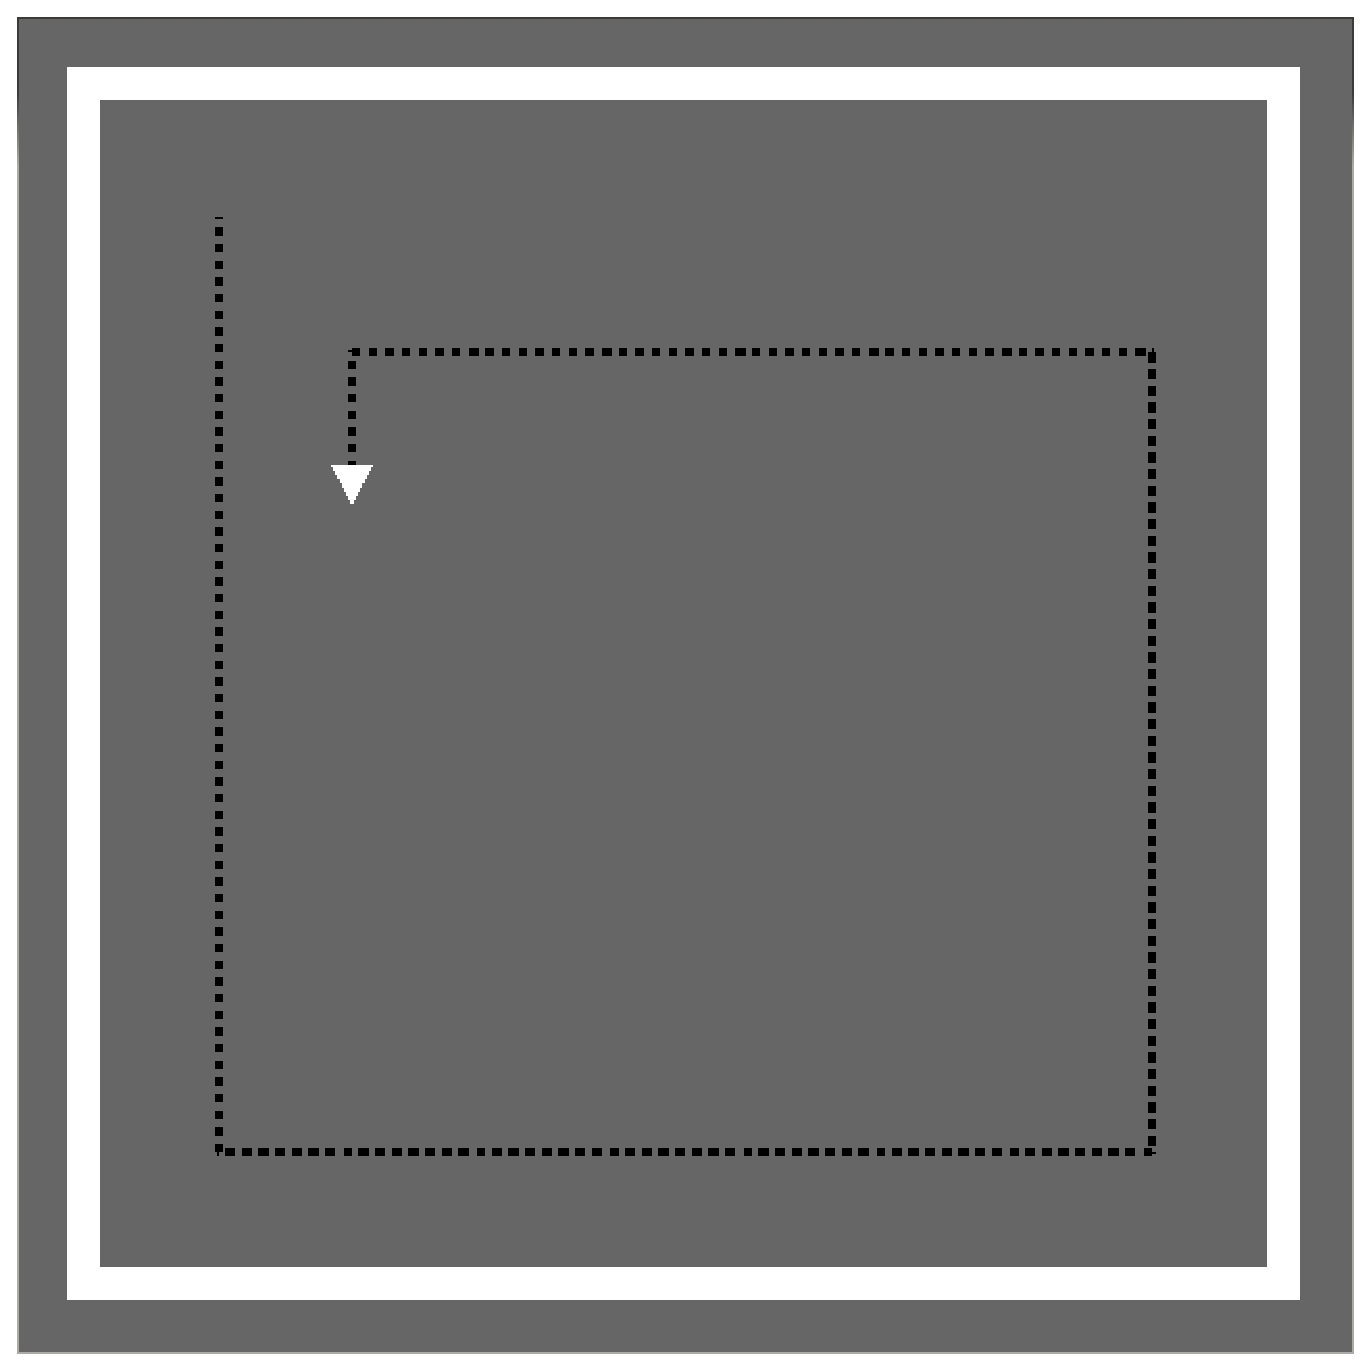
\includegraphics[width=.49\linewidth]{./spiral1}
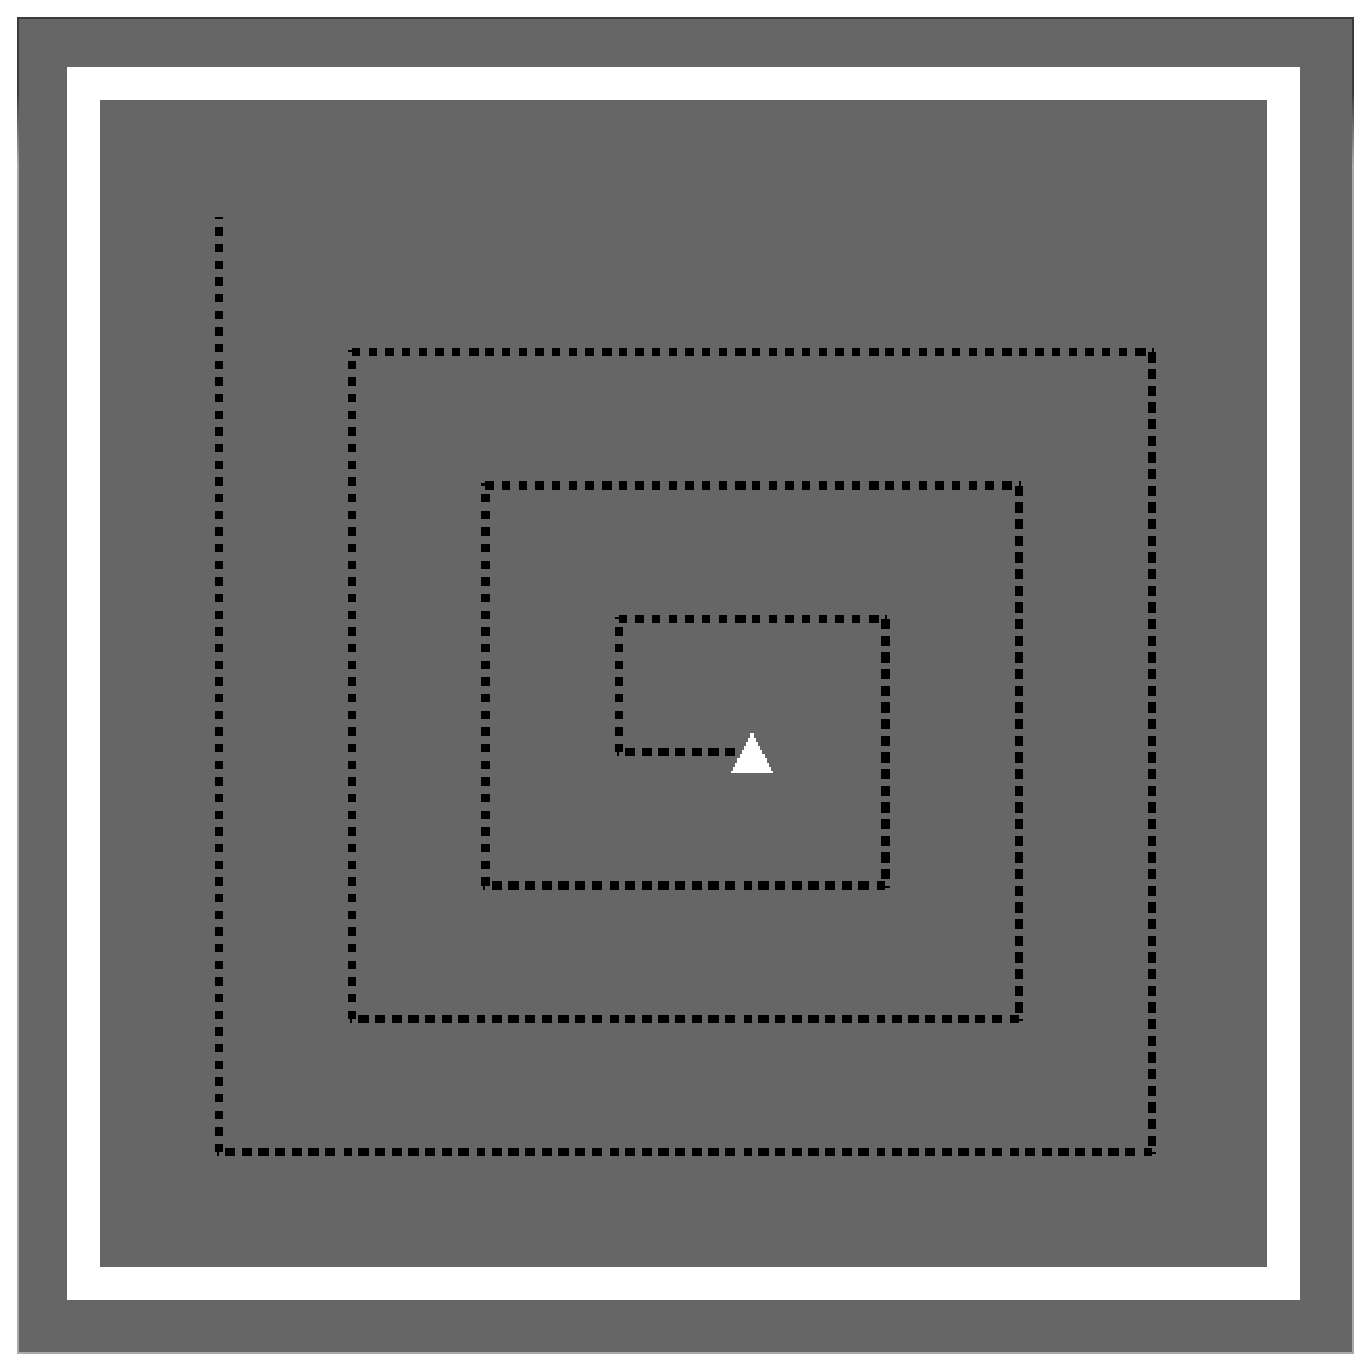
\includegraphics[width=.49\linewidth]{./spiral2}
\caption{Images generated by our robot simulator using the {\tt spiral} program.An important detail is that the robot simulator does not evaluate the Monadic program but rather executes a compiled first order representation of that program.}
\label{fig:spiral}
\end{figure}


\begin{figure}
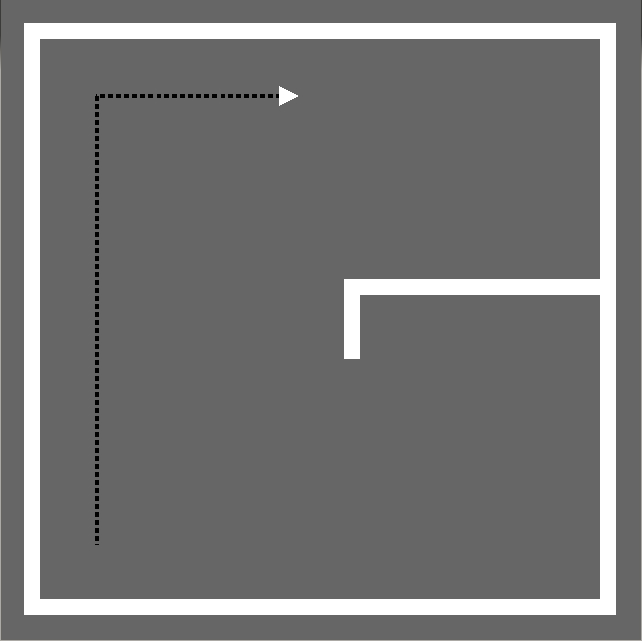
\includegraphics[width=.49\linewidth]{./wall1}
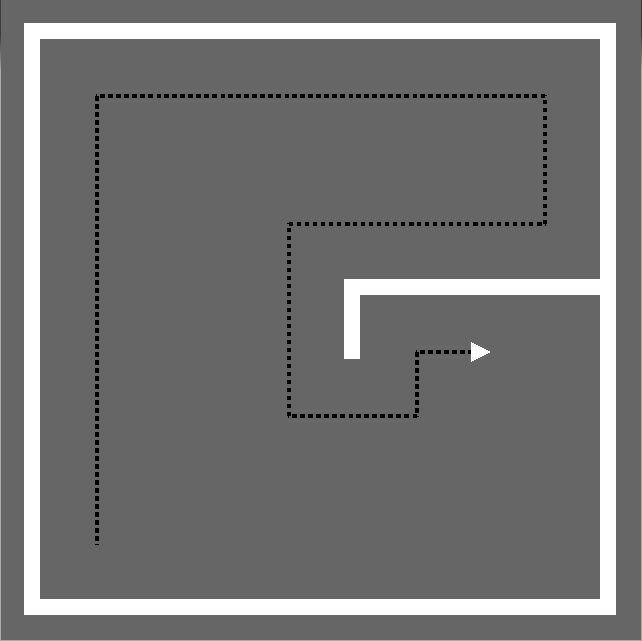
\includegraphics[width=.49\linewidth]{./wall2}
\caption{Images generated by the robot simulator using the {\tt followWall} program.}
\label{fig:followwall}
\end{figure}


%\subsection{Using Monads and do-notation} 

\FloatBarrier
\subsection{Implementation of the robot language}

\begin{small}
\begin{verbatim} 
data Program a where
  Move      :: Program ()
  TurnRight :: Program ()
  TurnLeft  :: Program ()

  Sensor    :: Program Exp

  Pen       :: Exp -> Program () 
  Cond      :: Exp 
            -> Program () 
            -> Program () 
            -> Program () 

  While     :: Program Exp 
            -> Program () 
            -> Program ()
   
  Return    :: a -> Program a 
  Bind      :: Program a 
            -> (a -> Program b) 
            -> Program b

\end{verbatim}
\end{small}

The \verb!Monad! instance. 

\begin{small}
\begin{verbatim} 
instance Monad Program where
  return = Return
  (>>=)  = Bind
\end{verbatim}
\end{small}

The expression type represent simple boolean expressions. It captures the 
operations we want to be able to perform on the input the robot gets from its 
sensor. 

\begin{small}
\begin{verbatim}
data Exp = Lit Bool
         | Var String
         | (:||:) Exp Exp
         | (:&&:)  Exp Exp
         | Not Exp  
\end{verbatim}
\end{small}

A possible extension to the capabilities of the robot would be to add integers
and arithmetic to the expression datatype. We leave this as an exercise to the 
reader. 

\begin{small}
\begin{verbatim} 
printExp :: Exp -> String
printExp (Lit b) = show b
printExp (Var nom) = nom
printExp (a :||: b) = "(" ++ printExp a   ++ 
                      " || "              ++ 
                      printExp b ++ ")"
printExp (a :&&: b) = "(" ++ printExp a   ++ 
                      " && "              ++ 
                      printExp b ++ ")"
printExp (Not a)    = "(" ++ "not" ++ " " ++ 
                      printExp a ++ ")"

instance Show Exp where
  show = printExp 
\end{verbatim} 
\end{small}

Given an {\em environment}, a map from names to booleans, it is also possible 
to evalute these expressions. 

\begin{small}
\begin{verbatim}
type Env = [(String, Bool)]

evalExp :: Env -> Exp -> Maybe Bool
evalExp e (Lit a) = Just a
evalExp e (Var str) = lookup str e
evalExp e (e1 :||: e2) = liftM2 (||) (evalExp e e1) 
                                     (evalExp e e2)
evalExp e (e1 :&&: e2) = liftM2 (&&) (evalExp e e1) 
                                     (evalExp e e2)
evalExp e (Not e1)     = liftM  not  (evalExp e e1)
\end{verbatim} 
\end{small}


\begin{itemize}
 \item Difference between {\tt Program Exp} and {\tt Exp}.
 \item {\tt Cond} takes {\tt Program ()}s and results in a {\tt Program ()} 
   if {\tt Cond} would have returned a {\tt Program a} we would be forced into 
   evaluation ``mode'' for conditionals. \newline 
   Another option is probably that we could have a 
   {\tt Cond :: Reifyable a => Exp -> Program a -> Program a -> Program a}. 
   Then some suitable {\tt Reifyable} class would be needed. 
\end{itemize} 


%maybe show evaluate in pieces! 
% Clean up the eval code and make sure it does what it should ! 

%Talk about eval and explain World and Grid and Robots ! 

\subsection{Evaluating programs} 

To be able to evaluate a robot program a world is needed. We consider the 
robot to be a part of this world. The robot moves around in a two dimensional 
grid of Cells. Each cell can contain either a wall or a ground.  

\begin{small}
\begin{verbatim}
data Cell = Wall | Ground 
\end{verbatim}
\end{small}

The grid is a two dimensional array of cells. 

\begin{small}
\begin{verbatim}
type Grid = Array (Int,Int) Cell
\end{verbatim}
\end{small}

There is a small set of operations defined on Grids. 

\begin{small}
\begin{verbatim}
size :: Grid -> (Int,Int) 
size = (\(x,y) -> (y,x)) .  snd  . bounds 

(*!) :: Grid -> (Int,Int) -> Cell
(*!) g (x,y) = (!) g (y,x)

fromList :: ((Int,Int),(Int,Int)) -> [Cell] -> Grid 
fromList = listArray
\end{verbatim}
\end{small}

More details! 

\begin{small}
\begin{verbatim} 
data Direction = North | South | East | West

type Pos       = (Int,Int)

type Line      = (Pos,Pos)  
                        
data World     = World { robotDir   :: Direction, 
                         robotPos   :: Pos,
                         robotPen   :: Bool,
                         robotEnv   :: Env,
                         robotTrack :: [Line],
                         worldGrid  :: Grid}
                 deriving Show 
\end{verbatim}
\end{small}

If the result we are interested in is the state of the world after 
executing a robot program, we can define an eval function as follows

\begin{small}
\begin{verbatim} 
eval :: Program a -> World -> World 
eval p w = snd $ eval' s p w
  where
    s = unsafePerformIO $ newEnumSupply

mkName :: Supply Int -> String
mkName s = "v" ++ show (supplyValue s)
\end{verbatim}
\end{small}

The big part of the evaluation process is performed by the {\tt eval'} function 
that has the signature \newline 
\verb!Supply Int -> Program a -> World -> (a,World)!. The evaluation function is simple.  
% NOTE: it is not in the evaluation function that problems occur.

\begin{small}
\begin{verbatim}
eval' :: Supply Int -> Program a -> World -> (a,World)  
eval' s Move w = ((), w')
  where
    w' = w {robotPos = tPos (robotDir w) (robotPos w)}

eval' s TurnRight w = ((), w')
  where
    w' = w {robotDir = turnR (robotDir w)}
eval' s TurnLeft w = ((), w')
  where
    w' = w {robotDir = turnL (robotDir w)}
    
eval' s Sensor w = (Var nom,w') 
  where
    cell = worldGrid w *! sensorPos 
    sensorPos = tPos (robotDir w) (robotPos w)
    env' = (nom,cell == Wall) : robotEnv w
    w'   = w { robotEnv = env' } 
    nom = mkName s
    
eval' s (Cond b p1 p2) w =
  case evalExp (robotEnv w) b  of
    (Just True) -> eval' s p1 w
    (Just False) -> eval' s p2 w
    Nothing -> error "eval': faulty robotEnv" 
    
eval' s (Pen b) w = ((),w') 
  where
    b' = evalExp (robotEnv w) b 
    w' = w {robotPen = fromJust b'}
    
eval' s (Return a) w = (a,w)
eval' s (Bind a f) w = (b,w2) 
  where
    (s1,s2) = split2 s
    (a1,w1) = eval' s1 a w
    (b,w2)  = eval' s2 (f a1) w1

 
tPos :: Direction -> Pos -> Pos    
tPos North (x,y) = (x,y-1)
tPos South (x,y) = (x,y+1)
tPos East  (x,y) = (x+1,y)
tPos West  (x,y) = (x-1,y)

turnR :: Direction -> Direction 
turnR North = East
turnR East = South
turnR South = West
turnR West = North

turnL = turnR . turnR . turnR   
\end{verbatim}
\end{small}

\subsection{Printing and compiling programs} 
This is where it gets interesting. 

\begin{small}
\begin{verbatim}
printPrg :: Program a -> String
printPrg p = snd $ printPrg' s p
  where
    s = unsafePerformIO $ newEnumSupply

printPrg' :: Supply Int -> Program a -> (a, String)
printPrg' s Move = ((),"move\n")
printPrg' s TurnRight = ((),"turnR\n")
printPrg' s TurnLeft = ((),"turnL\n")
printPrg' s Sensor = (Var nom,nom ++ " <- sensor\n")
  where
    nom = mkName s
printPrg' s (Cond b p1 p2) = ((),str)
  where str = "if " ++ printExp b ++ "\n" ++
              "then\n" ++ snd (printPrg' s p1) ++ 
              "else\n" ++ snd (printPrg' s p2)
printPrg' s (While pb p) = ((),str)
  where
    (s1,s2) = split2 s 
    str = "while {" ++ snd (printPrg' s1 pb) ++ "}\n" ++
          "do\n" ++ 
          snd (printPrg' s1 p) ++ 
          "done\n"
printPrg' s (Pen b)  = ((),str)
  where
    str = "setPen " ++ printExp b ++ "\n"
printPrg' s (Return a) = (a, "")
printPrg' s (Bind pa f) = (b,str ++ str2) 
  where
    (s1,s2) = split2 s 
    (a,str) = printPrg' s1 pa 
    prg2 = f a
    (b,str2) = printPrg' s2 prg2

\end{verbatim}
\end{small}

%\subsection{Infinite programs}
%The spiral program can not easily be compiled.  
%
%\begin{verbatim}
%spiral n = do 
%  repeat n Move 
%  TurnLeft 
%  spiral (n+1) 
%\end{verbatim} 
%
%propose a method to compile it anyway (in stages, using lazyness). 



%\begin{figure}
%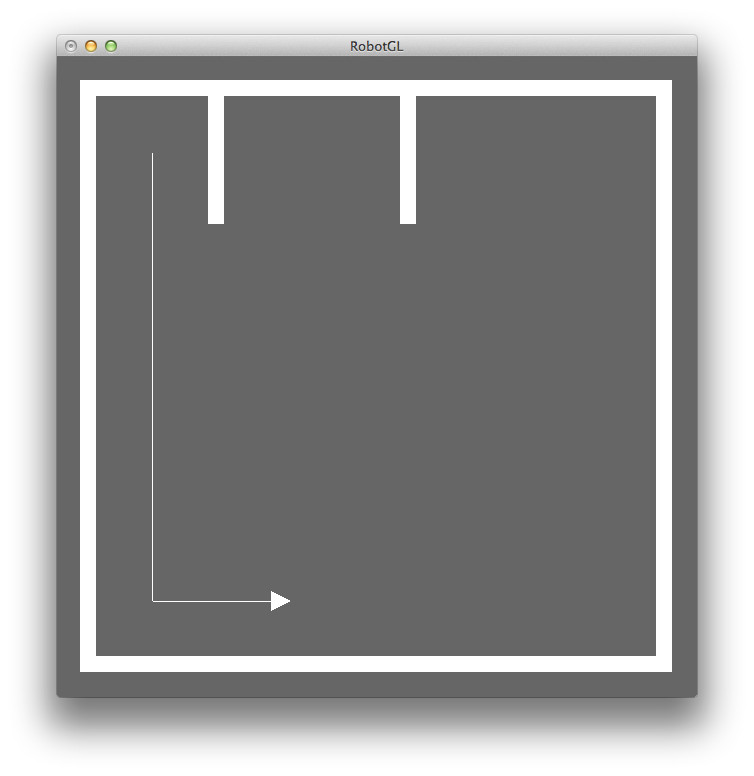
\includegraphics[width=5cm]{./robot1}
%\caption{example robot graphics}
%\label{fig:ROBOT1}

%\end{figure}


%\begin{figure}[ht]
% \begin{minipage}[b]{0.45\linewidth}
%
%   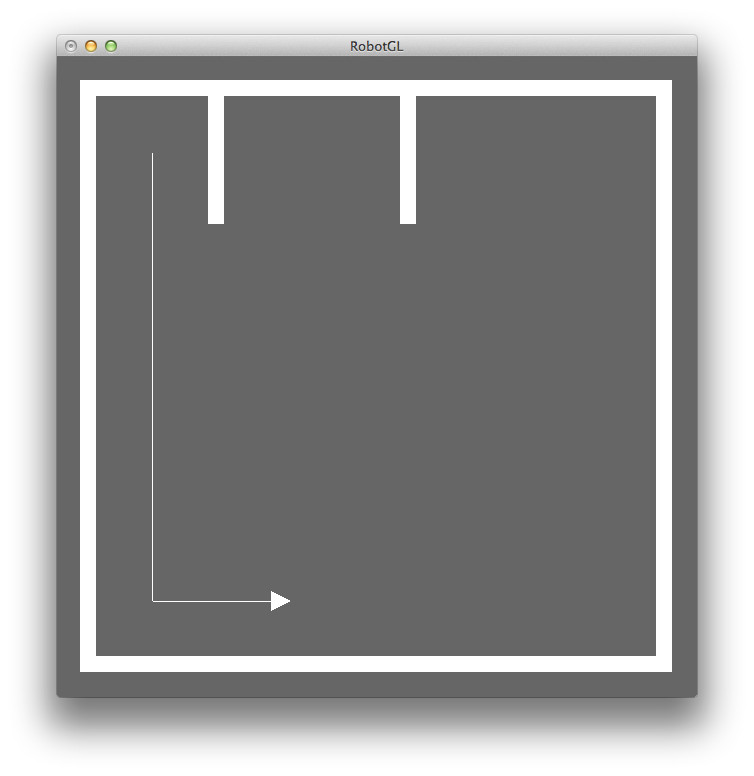
\includegraphics[width=\textwidth]{./robot1}
%   %\caption{example robot graphics}
%   %\label{fig:ROBOT1}
%  \end{minipage}
%
%
%  \begin{minipage}[b]{0.45\linewidth}
%   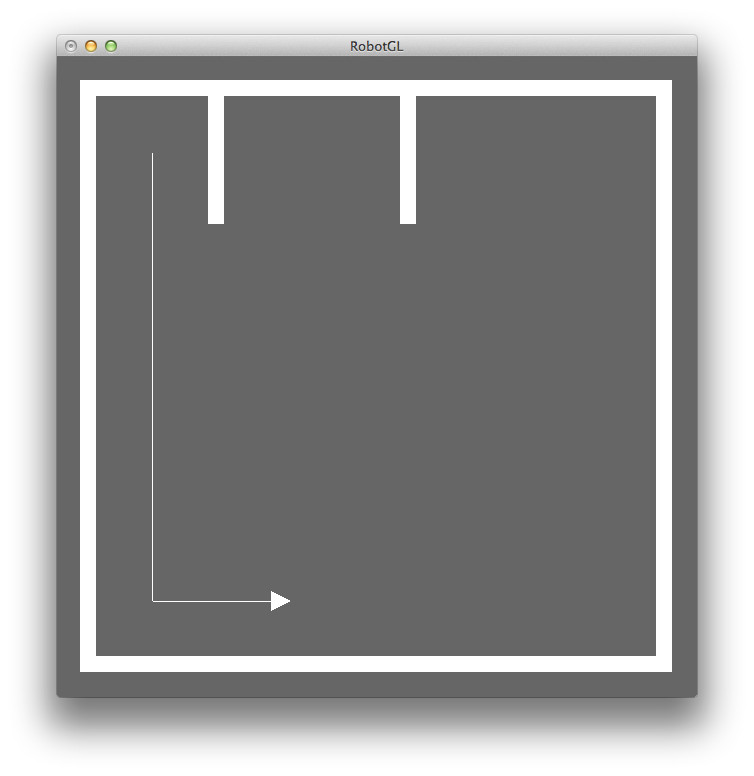
\includegraphics[width=\textwidth]{./robot1}
%   %\caption{example robot graphics}
%   %\label{fig:ROBOT1}
%  \end{minipage}
%\end{figure}


%\begin{figure}
%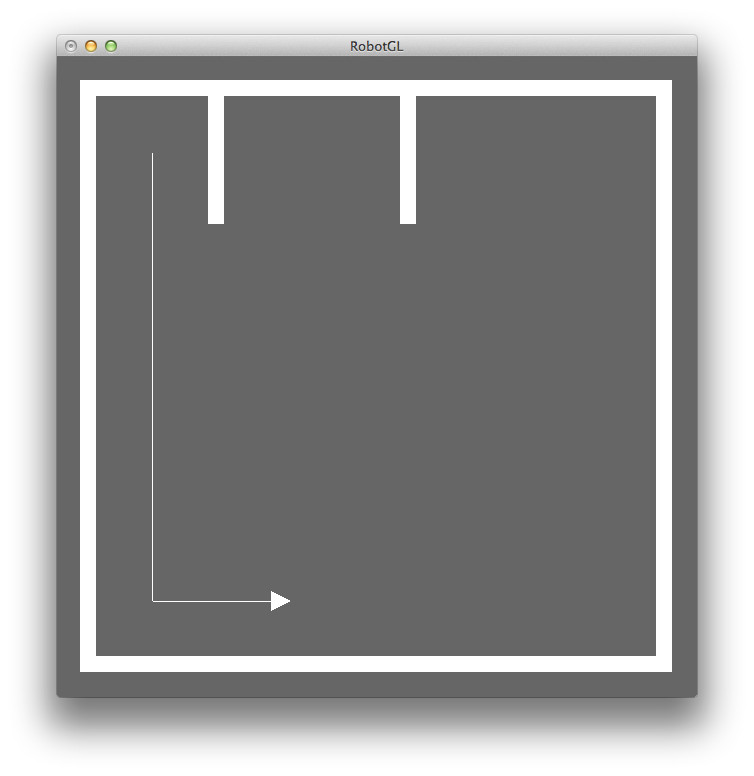
\includegraphics[width=.5\linewidth]{./robot1}
%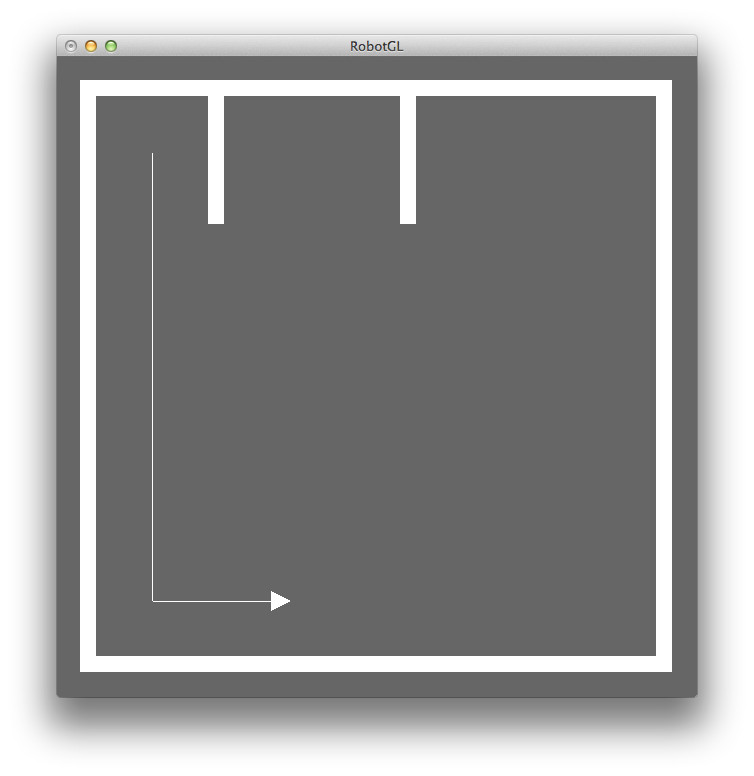
\includegraphics[width=.5\linewidth]{./robot1}
%\caption{two images  }
%\label{fig:robo}
%\end{figure}
